\documentclass[aspectratio=169,11pt]{beamer}
\usepackage[T1]{fontenc}
\usepackage{lmodern,amsmath,amssymb,mathtools,bm,booktabs,array,graphicx,tikz}
\usetikzlibrary{arrows.meta,positioning,calc,decorations.pathreplacing,patterns}
\definecolor{ink}{HTML}{17344D}\definecolor{accent}{HTML}{087E8B}\definecolor{pale}{HTML}{EDF5F5}\definecolor{gold}{HTML}{AD6B19}
\providecommand{\dd}{\,\mathrm{d}}\providecommand{\R}{\mathbb{R}}
\providecommand{\E}{\mathbb{E}}\providecommand{\Var}{\operatorname{Var}}
\providecommand{\Cov}{\operatorname{Cov}}\providecommand{\diag}{\operatorname{diag}}
\providecommand{\norm}[1]{\left\lVert#1\right\rVert}
\providecommand{\abs}[1]{\left|#1\right|}
\usefonttheme{professionalfonts}
\setbeamercolor{normal text}{fg=black,bg=white}
\setbeamercolor{frametitle}{fg=ink,bg=white}
\setbeamercolor{title}{fg=ink}\setbeamercolor{structure}{fg=accent}
\setbeamercolor{block title}{fg=ink,bg=pale}\setbeamercolor{block body}{fg=black,bg=pale!40}
\setbeamercolor{alerted text}{fg=accent}
\setbeamerfont{frametitle}{size=\Large,series=\bfseries}
\setbeamerfont{title}{size=\LARGE,series=\bfseries}
\setbeamertemplate{navigation symbols}{}
\setbeamersize{text margin left=.7cm,text margin right=.7cm}
\setbeamertemplate{frametitle}{\vspace{.18cm}\insertframetitle\par\vspace{.1cm}{\color{accent}\hrule height .6pt}\vspace{.12cm}}
\newcommand{\notestarget}{notes.pdf}\newcommand{\noteslabel}{Notes}
\setbeamertemplate{footline}{\hspace{.7cm}\color{ink}\scriptsize Mathematical Modeling\quad\href{\notestarget}{\noteslabel}\hfill\insertframenumber\,/\,\inserttotalframenumber\hspace{.7cm}\vspace{.18cm}}
\setbeamercovered{invisible}
\hypersetup{pdfauthor={Zan Ahmad},pdftitle={Finite-population genetics: inheritance, drift, and fixation},pdfpagemode=UseNone}
\begin{document}
\begin{frame}[plain]\vfill
{\small\color{accent} Mathematical Modeling \quad Lecture 7}\par\medskip
{\raggedright\hyphenpenalty=10000\exhyphenpenalty=10000\LARGE\bfseries\color{ink} Finite-population genetics: inheritance, drift, and fixation}\par\bigskip
Zan Ahmad\par\smallskip
{\small Fall 2024}\par\vfill\end{frame}
\renewcommand{\notestarget}{notes.pdf\#note-allele-counts-and-genotype-frequencies}
\begin{frame}[t,fragile,label=slide-diploid-accounting]{Diploid accounting}
\[n_{AA}+n_{AB}+n_{BB}=N,\qquad p=\frac{2n_{AA}+n_{AB}}{2N}.\]\pause{} Every heterozygote contributes one $A$ copy and one $B$ copy.
\end{frame}
\renewcommand{\notestarget}{notes.pdf\#note-random-pairing-and-hardy-weinberg-probabilities}
\begin{frame}[label=slide-independent-gamete-pairing-figure]{Independent gamete pairing}
\centering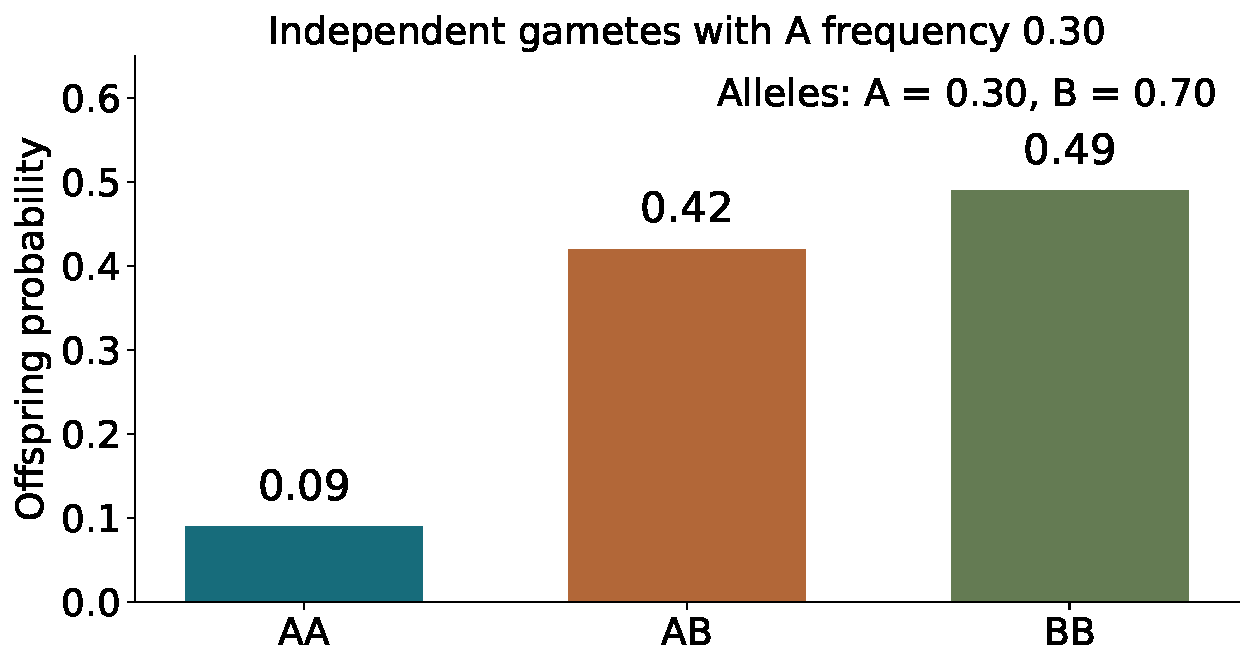
\includegraphics[width=.98\linewidth,height=.69\textheight,keepaspectratio]{genotype-probabilities.pdf}\end{frame}
\renewcommand{\notestarget}{notes.pdf\#note-random-pairing-and-hardy-weinberg-probabilities}
\begin{frame}[t,fragile,label=slide-independent-gamete-pairing]{Independent gamete pairing}
\[\Pr(AA)=p^2,\quad \Pr(AB)=2p(1-p),\quad\Pr(BB)=(1-p)^2.\]\pause{} The heterozygote combines two ordered outcomes.
\end{frame}
\renewcommand{\notestarget}{notes.pdf\#note-random-pairing-and-hardy-weinberg-probabilities}
\begin{frame}[t,fragile,label=slide-probabilities-and-expected-counts]{Probabilities and expected counts}
At $p=0.30$:\[(p^2,2p(1-p),(1-p)^2)=(0.09,0.42,0.49).\]\pause{} For $100$ offspring, expected counts are $(9,42,49)$.\par\medskip A finite random sample need not equal its expected counts.
\end{frame}
\renewcommand{\notestarget}{notes.pdf\#note-random-pairing-and-hardy-weinberg-probabilities}
\begin{frame}[t,fragile,label=slide-neutrality-preserves-the-expected-allele-fraction]{Neutrality preserves the expected allele fraction}
\[p^2+\frac12\,2p(1-p)=p.\]\pause{} No selection, mutation, or migration is included.\par\medskip Constancy of expectation does not imply constancy of each realization.
\end{frame}
\renewcommand{\notestarget}{notes.pdf\#note-the-neutral-finite-population-transition-law}
\begin{frame}[t,fragile,label=slide-a-finite-state-variable]{A finite state variable}
\[K_n\in\{0,1,\ldots,2N\},\qquad p_n=K_n/(2N).\]\pause{} Offspring copies are sampled from the current parental pool.
\end{frame}
\renewcommand{\notestarget}{notes.pdf\#note-the-neutral-finite-population-transition-law}
\begin{frame}[t,fragile,label=slide-the-binomial-transition-law]{The binomial transition law}
\[K_{n+1}\mid p_n\sim\operatorname{Binomial}(2N,p_n).\]\pause{}\[P_{ij}=\binom{2N}{j}(i/2N)^j(1-i/2N)^{2N-j}.\]
\end{frame}
\renewcommand{\notestarget}{notes.pdf\#note-the-neutral-finite-population-transition-law}
\begin{frame}[t,fragile,label=slide-one-neutral-generation]{One neutral generation}
\[N=25,\quad K_n=15\quad\Rightarrow\quad p_n=0.30.\]\pause{} A possible next count is $K_{n+1}=18$, giving $p_{n+1}=0.36$.\par\medskip The next generation samples with probability $0.36$.
\end{frame}
\renewcommand{\notestarget}{notes.pdf\#note-conditional-moments-and-accumulation-of-drift}
\begin{frame}[t,fragile,label=slide-conditional-expectation-and-variance]{Conditional expectation and variance}
\[\mathbb E[p_{n+1}\mid p_n]=p_n,\qquad\operatorname{Var}(p_{n+1}\mid p_n)=\frac{p_n(1-p_n)}{2N}.\]\pause{} Mean change is zero; random change need not be zero.
\end{frame}
\renewcommand{\notestarget}{notes.pdf\#note-conditional-moments-and-accumulation-of-drift}
\begin{frame}[t,fragile,label=slide-population-size-scaling-of-fluctuations]{Population-size scaling of fluctuations}
At $p=0.30$:\[\sigma_{25}=\sqrt{0.21/50}\simeq0.06481,\qquad\sigma_{250}=\sqrt{0.21/500}\simeq0.02049.\]\pause{} Tenfold larger $N$ reduces standard deviation by $\sqrt{10}$.
\end{frame}
\renewcommand{\notestarget}{notes.pdf\#note-conditional-moments-and-accumulation-of-drift}
\begin{frame}[label=slide-a-constant-ensemble-mean-figure]{A constant ensemble mean}
\centering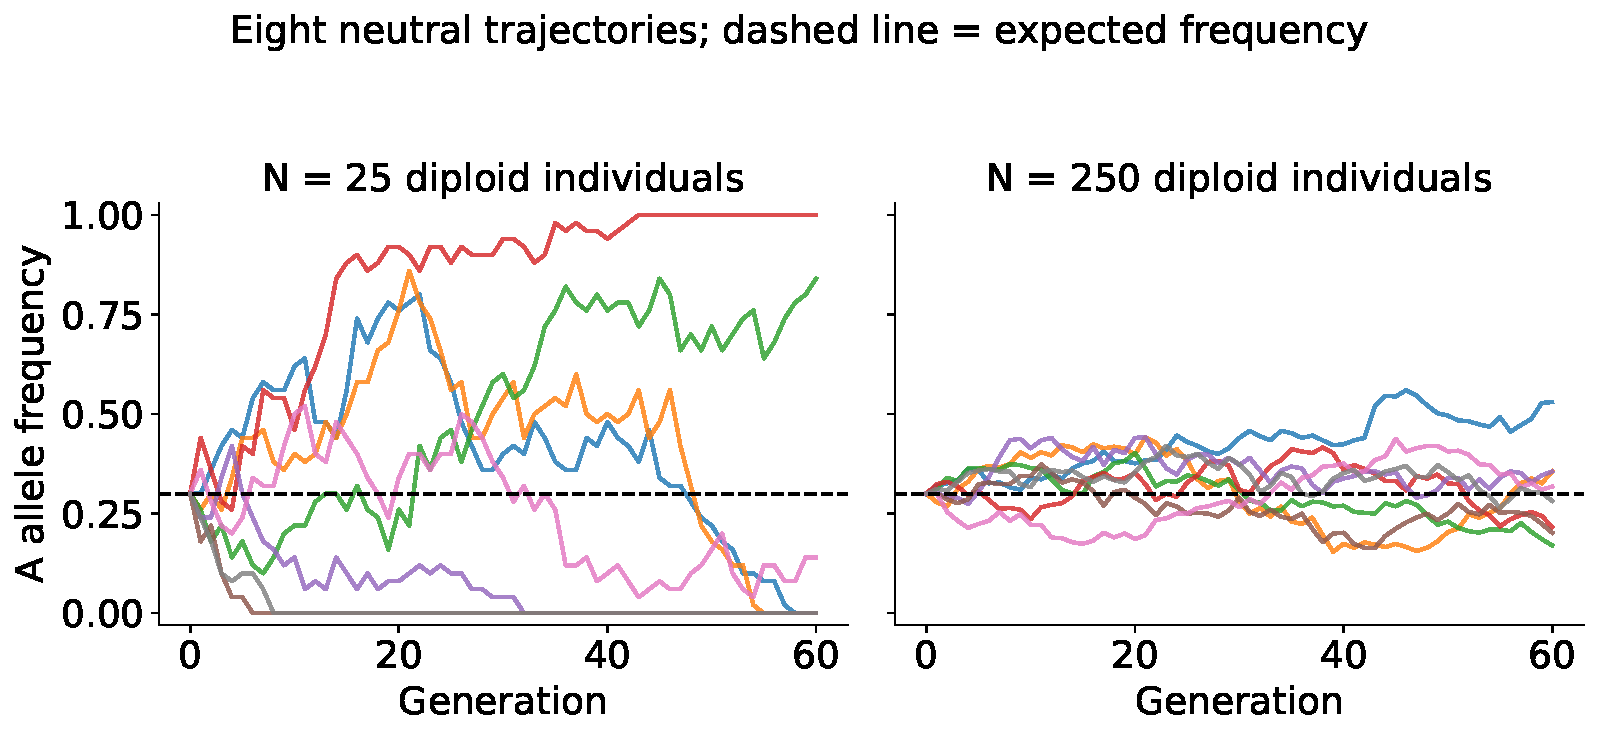
\includegraphics[width=.98\linewidth,height=.69\textheight,keepaspectratio]{neutral-drift.pdf}\end{frame}
\renewcommand{\notestarget}{notes.pdf\#note-conditional-moments-and-accumulation-of-drift}
\begin{frame}[t,fragile,label=slide-a-constant-ensemble-mean]{A constant ensemble mean}
\[\mathbb E[p_{n+1}]=\mathbb E[\mathbb E[p_{n+1}\mid p_n]]=\mathbb E[p_n]=p_0.\]\pause{} The plotted dashed line is $p_0$, not the mean of eight displayed runs.
\end{frame}
\renewcommand{\notestarget}{notes.pdf\#note-conditional-moments-and-accumulation-of-drift}
\begin{frame}[t,fragile,label=slide-expected-heterozygosity-declines]{Expected heterozygosity declines}
\[\mathbb E[p_{n+1}(1-p_{n+1})\mid p_n]=\left(1-\frac1{2N}\right)p_n(1-p_n).\]\pause{}\[\mathbb E[H_n]=2p_0(1-p_0)\left(1-\frac1{2N}\right)^n.\]
\end{frame}
\renewcommand{\notestarget}{notes.pdf\#note-conditional-moments-and-accumulation-of-drift}
\begin{frame}[t,fragile,label=slide-distributional-broadening]{Distributional broadening}
\[\operatorname{Var}(p_n)=p_0(1-p_0)\left[1-\left(1-\frac1{2N}\right)^n\right].\]\pause{} The mean is fixed while probability moves toward the endpoints.
\end{frame}
\renewcommand{\notestarget}{notes.pdf\#note-absorption-and-fixation-probability}
\begin{frame}[t,fragile,label=slide-absorbing-endpoints]{Absorbing endpoints}
\[p_n=0\Rightarrow p_{n+1}=0,\qquad p_n=1\Rightarrow p_{n+1}=1.\]\pause{} Without mutation or migration, a missing allele cannot be resampled.
\end{frame}
\renewcommand{\notestarget}{notes.pdf\#note-absorption-and-fixation-probability}
\begin{frame}[t,fragile,label=slide-neutral-fixation-probability]{Neutral fixation probability}
For a finite neutral chain, absorption occurs with probability one.\pause{}\[\Pr(p_\infty=1)=\mathbb E[p_\infty]=p_0.\] Fixation does not require a selective advantage.
\end{frame}
\renewcommand{\notestarget}{notes.pdf\#note-simulation-reproducibility-and-stochastic-verification}
\begin{frame}[t,fragile,label=slide-computational-checks-for-a-random-model]{Computational checks for a random model}
Check integer counts, the $1/(2N)$ frequency grid, bounds, and absorbing states.\pause{}\par\medskip Compare repeated-draw moments with theoretical moments using sampling uncertainty.\par\medskip A seed controls repeatability, not representativeness.
\end{frame}
\renewcommand{\notestarget}{notes.pdf\#note-simulation-reproducibility-and-stochastic-verification}
\begin{frame}[t,fragile,label=slide-mean-dynamics-and-individual-populations]{Mean dynamics and individual populations}
\[p_{n+1}=p_n\] reproduces the neutral expectation but removes all sampling variation.\pause{}\par\medskip Drift, loss, and fixation require the distributional model.
\end{frame}
\end{document}
